\documentclass[a4paper,11pt,twocolumn]{article}

\usepackage{icphs2023}
\usepackage{metalogo} % Only needed for the XeLaTeX logo
\usepackage{epstopdf}
\usepackage{graphicx}
\usepackage{adjustbox}
\usepackage{float}
\usepackage[section]{placeins}
\usepackage{multirow}
\graphicspath{{images/}}
\usepackage{subcaption}
%\usepackage[style=authoryear]{biblatex}
%\renewcommand*{\nameyeardelim}{\addcomma\addspace}

\usepackage{booktabs}
\usepackage[scale=2]{ccicons}

\usepackage{tipa}
\newcommand{\nt}[1]{\textipa{[#1]}} % narrow transcription
\newcommand{\wt}[1]{\textipa{/#1/}} % wide transcription

\hyphenpenalty=10000 % no hyphenation

\title{Coarticulation and contrast in a vowel harmony system: coarticulatory propensity in Khalkha Mongolian V-C-V sequences}
\author{XXX}
\organization{XXX}
\email{XXX}
\begin{document}
	
	\maketitle
	
	\begin{abstract}
		In Khalkha Mongolian, vowels in non-compound words share the features [ATR] and [round], harmony operating in the carryover (left-to-right) direction. The high-front vowel /i/ does not participate in harmony, giving ``non-harmonic'' VCV sequences. Vowel harmony has been variously understood to emerge (i) when listeners fail to perceptually compensate for acoustic variation due to coarticulation, and (ii) for perceptual advantage in perceptually "weak" contrasts. Towards understanding the relationship between these processes, we quantify coarticulatory variation by comparing dependencies in first- and second-formant frequencies (F1\&F2) of vowels in harmonic vs non-harmonic VCV sequences. Unlike harmonic sequences, non-harmonic sequences demonstrate greater coarticulation in the anticipatory (right-to-left) direction---opposite to that of vowel harmony. /i/, which is transparent to harmony, demonstrates high coarticulatory resistance. We argue that in systems where vowel harmony is well-established, synchronic patterns of coarticulatory propensity serve to limit feature-sharing in non-harmonic sequences. We relate this to the notion of contrast preservation.
	\end{abstract}
	
	\keywords{Khalkha Mongolian, vowel harmony, coarticulation, vowels, formants}
	
	
	\section{Coarticulation and Vowel harmony}
	
	Vowel harmony is a grammatical feature of languages whereby sequences of vowels (contiguous or non-contiguous) within a certain domain, e.g. the word, obligatorily have the same value for certain phonological features. This is a productive rule, and leads to predictable variation of vowels depending on phonological context. This could be left-to-right: \emph{carryover}, where features of a preceding vowel affect those of the following vowels, or right-to-left: \emph{anticipatory} where the converse happens. Independent of this grammatical process, one feature of speech is that sounds are not produced in discrete sequences. Rather, articulatory gestures overlap during connected speech, and this kind of \emph{coarticulation} results in acoustic variation. Coarticulation could be carryover when the gestures of an earlier target perturb the latter in a mechanico-inertial fashion, or anticipatory, where articulatory planning for a subsequent vowel affects the production of an earlier vowel, and is frequently both simultaneously. To extract stable phonological categories from such a variable signal, listeners must perceptually compensate for the acoustic variation resulting from coarticulation. Given the parallels between this kind of physiological-psychoacoustic process and grammatical harmony processes, vowel harmony has been understood to diachronically emerge when listeners fail to perceptually compensate for acoustic variation due to coarticulation \cite{ohala1994,beddor2002}, eventually perceiving the coarticulated variation as part of the phonological feature of the category. Under this hypothesis, the greater persistence of mechanico-inertial/carryover coarticulation would give rise to carryover harmony, while the persistence of anticipatory coarticulation leads to right-to-left harmony systems. An important aspect to remember is that coarticulation is assumed to be a non-voluntary by-product of articulation, and therefore continues to exist even after harmony has developed. Assuming the hypothesis of causation, once a psycho-acoustic process such as the perceptual persistence of e.g. carryover coarticulation has been set in motion, what prevents the system from further coarticulation, assimilating more features, and eventually resorting to a radical process of vowel copying? While systems with phonological vowel-copying exist (e.g. Telugu; \cite{dutta2016}), other harmony systems appear to be in a synchronic state of equilibrium, where harmony operates over certain features and segments, but not others. Specifically, most harmony systems also contain some form of \emph{non-harmony}-- sequences or segments that do not participate in harmony, either by completely ignoring it (transparent segments), or blocking it (opaque segments). Setting aside the issue of which specific sequences emerge as non-harmonic diachronically, how do such sequences persist in synchronic systems, given the continued existence of coarticulation in the direction of harmony, and the system's proclivity for its perceptual non-compensation? In other words, what checks does the language system put in place to prevent the spillover of the very processes that initiated harmony, into its grammatically non-harmonic domains?
	
	Towards understanding this, our project examines how coarticulation functions within a system with well-established and robust vowel harmony. We measure the acoustic consequences of coarticulation in harmonic and non-harmonic sequences, and compare the patterns of coarticulatory propensity in these sequences.  
	
	
	\section{Vowel system of Khalkha Mongolian}
	Khalkha Mongolian has seven phonological vowel categories, classified as non-pharyngeal (+ATR) and pharyngeal (-ATR) \cite{svantesson2005}: 
	\begin{table}[!h]
		\begin{center}
			\small
			\begin{tabular}{@{}cccc@{}}
				\toprule 
				& [+ATR] & [-ATR]     & neutral                \\ \midrule
				high     & \textipa{u}                  & \textipa{U}    & \textipa{i} \\
				non-high & \textipa{e, o}               & \textipa{a}, \textipa{O} &                        \\ \bottomrule
			\end{tabular}%
			\caption{Monopthongs in Khalkha Mongolian, classified by harmony class}
			\label{table_vowels}
		\end{center}
	\end{table}     
	
	
	\begin{itemize}
		\item Non-high vowels have rounded (right) and non-rounded (left) counterparts
		\item /i/ has 2 allophones: \nt{i} in ATR words, \nt{I} in non-ATR words
	\end{itemize}
	
	\begin{itemize} 
		\item \textbf{Vowel harmony:} vowels in non-compound words must share the feature [ATR]. A subset of vowels (non-high: \textipa{e, o, a, O}) show rounding harmony.
		\item Focus of present study: ATR harmony
		\item \textbf{Directionality:} left-to-right
		\item \nt{i} is `transparent' to harmony, resulting in non-harmonic sequences
		
	\end{itemize}
	
	
	\subsection{Questions and Hypotheses}
	
	We focus on ATR harmony, whose acoustic correlates are the first and second formant frequencies (F1 and F2), and operationalize coarticulation as variability and dependency along those acoustic features. 
	
	We ask whether the extent and directionality of coarticulation differ between harmonic and non-harmonic VCV sequences. We expect that if the system actively preserves non-harmony in certain domains, such sequences will differ in coarticulatory patterns, compared to domains in which harmony has developed (diachronically) as a result of coarticulation. 
	
	\section{Materials and Methods}
	
	\subsection{Materials}
	We recorded 14 female native speakers reading 4 repetitions of 59 target words, in the frame [pi X gesen] ``I said X'' (critical items: 59$\times$14$\times$4 = 3304). Targets were disyllabic words of the form (C)V1CV2(C) \cite{svantesson2005}, and each vowel occurred in both initial (v1) and non-initial (V2) position. Words in which \wt{i} occupied the V2 position were classified as ``non-harmonic'', and all other words as ``harmonic''.
	
	\subsection{Acoustic analysis}
	A subset of recordings was used to train an acoustic model with the Montreal Forced Aligner \cite{mcauliffe2017montreal} to segment and annotate the data. We analyze Lobanov-normalized F1 and F2 at vowel midpoints. To quantify coarticulatory propensity, we use linear mixed effects models to examine how well the identity of V2 explains variance in the acoustics of V1 (anticipatory coarticulation) and vice-versa (carryover coarticulation).
	
	\section{Results}
	\subsection{Vowel space diffusion}
	Plotting F1 and F2 values of vowels in the initial (V1) and non-initial (V2) position (figure \ref{figure_combined}) shows the following patterns: for harmonic sequences, the vowel space for V2 is more diffused than V1, suggesting greater variability due to coarticulation. Since the V2 position in non-harmonic sequences can be occupied only by a subset of the vowel space, and is in complementary distribution to V1, the plot of the V2 vowel space of non-harmonic sequences is not informative. However, the vowel space for V1 shows that the low front vowel \wt{a} and the high back vowel \wt{u} are noticeably more diffused in the initial position of a non-harmonic sequence, compared to a harmonic sequence. This suggests differences in patterns of variability between the two groups. This is probed in the statistical analyses. 
	
	\begin{center}
		\begin{figure}[!ht]
			\begin{subfigure}[t]{0.2\textwidth}
				\centering
				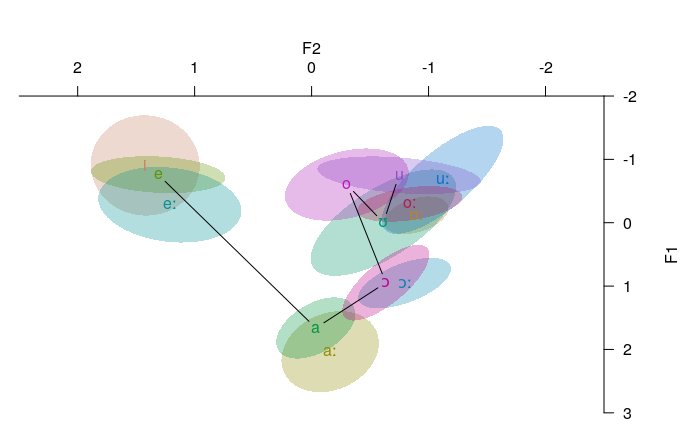
\includegraphics[scale=0.2]{har_v1.png} 
				\caption{harmonic subset: V$_1$} \label{har_v1}
			\end{subfigure}
			\begin{subfigure}[t]{0.2\textwidth}
				\centering
				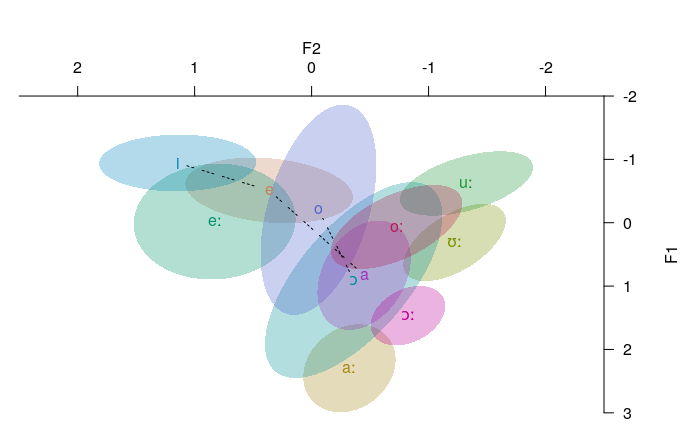
\includegraphics[scale=0.2]{har_v2.png} 
				\caption{harmonic subset: V$_2$} \label{har_v2}
			\end{subfigure}	
			\begin{subfigure}[t]{0.2\textwidth}
				\centering
				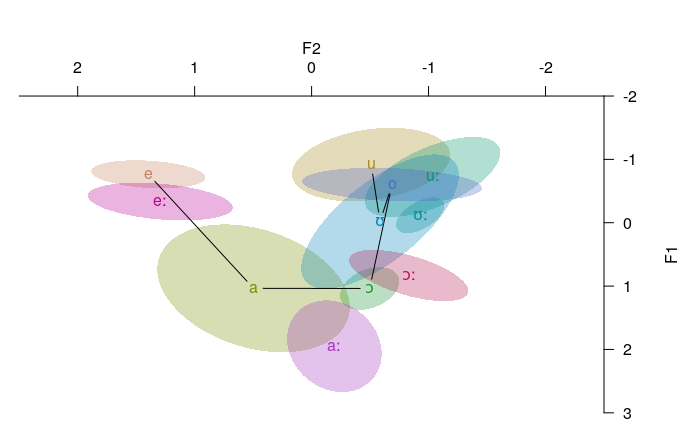
\includegraphics[scale=0.2]{nh_v1.png} 
				\caption{non-harmonic: V$_1$} \label{nh_v1}
			\end{subfigure}
			\begin{subfigure}[t]{0.2\textwidth}
				\centering
				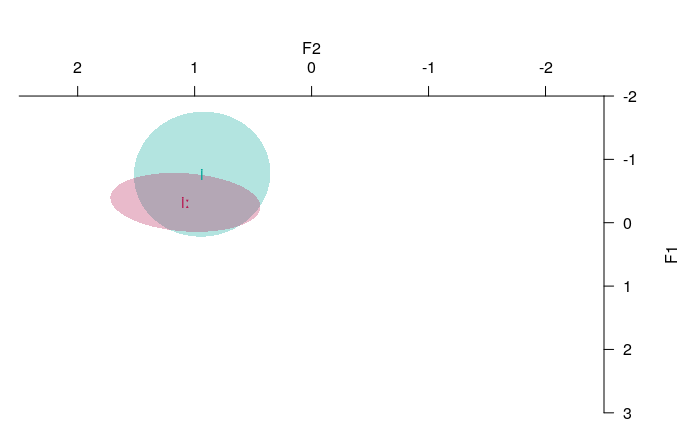
\includegraphics[scale=0.2]{nh_v2.png} 
				\caption{non-harmonic: V$_2$} \label{nh_v2}
			\end{subfigure}
			\caption{Steady-state formants for harmonic and non-harmonic vowel sequences}
			\label{figure_combined}
		\end{figure}
	\end{center}
	\FloatBarrier
	
	\subsection{Statistical analyses}
	For any vowel, we expect F1 and F2 values to be predicted by the phonological identity of the vowel. To quantify coarticulation, we used mixed effects models \cite{lme4} in R \cite{R-Core-Team:2015aa} to probe how well the formant frequency of a segment is predicted by the identity of the other vowel in the word, giving a measure of coarticulatory variability. Moreover, we examine whether this tendency differs between harmonic and non-harmonic words by comparing effect sizes of the explanatory variable in each model using the \textit{effectsize}  package \cite{effectsize} in R. The following sections summarize the results for F1 and F2 respectively. For all models, data was mean-centered and scaled prior to analysis to increase the likelihood of convergence \cite{bates2015}. In all cases, the random effects were ..., except for the ... sequences, where the random effect structure was simplified to ... to make the model converge.
	
	\subsubsection{F1}
	
	\begin{table}[h]
		\adjustbox{max width=0.45\textwidth}{
			\begin{tabular}{@{}lllllll@{}}
				\toprule
				Harmony type & Direction & Model fixed effects & ChiSq & Df & p & effect size ($\eta^2$) \footnote{using the effectsize package in R \cite{effectsize}} \\ \midrule
				harmonic     & anticipatory & F1V1t5 $\sim$ V1+\textbf{V2} & 17.174 & 9  & 0.04606 *     & 0.322 \\
				& carryover    & F1V2t5 $\sim$ V2+\textbf{V1} & 34.131 & 11 & 0.003443 *** & 0.536 \\ \midrule
				non-harmonic & anticipatory & F1V1t5 $\sim$ V1+\textbf{V2} & 100.87 & 1  & < 2.2e-16 *** & 0.133 \\
				& carryover    & F1V2t5 $\sim$ V2+\textbf{V1} & 133.41 & 10 & < 2.2e-16 *** & 0.174
			\end{tabular}%
		}
		\caption{Model outputs for coarticulation in F1, compared to a null model lacking the explanatory variable (bold)}
		\label{table_results_f1}
	\end{table}
	\FloatBarrier
	
	Table \ref{table_results_f1} summarizes the final model and output for F1. The results indicate robust coarticulation in both directions, with larger effects in the carryover (left-to-right) direction. 
	
	\subsubsection{F2}
	Table \ref{table_results_f2} summarizes the final model and output for F2. In the harmonic subset, coarticulation is primarily carryover (left-to-right). Anticipatory coarticulation is not statistically significant. In contrast, non-harmonic sequences show greater coarticulation in the anticipatory (right-to-left) direction. 
	
	\begin{table}[h]
		\adjustbox{max width=0.48\textwidth}{
			\begin{tabular}{@{}lllllll@{}}
				\toprule
				Harmony type &
				Direction &
				Model fixed effects &
				ChiSq &
				Df &
				p &
				effect size ($\eta^2$) \\ \midrule
				harmonic & anticipatory & F2V1t5 $\sim$ V1+\textbf{V2} & 9.3863 & 9  & 0.4024        & 0.191 \\
				& carryover    & F2V2t5 $\sim$ V2+\textbf{V1} & 22.79  & 11 & 0.01892 *     & 0.404 \\ \midrule
				non-harmonic &
				anticipatory &
				F2V1t5 $\sim$ V1+\textbf{V2} &
				110.57 &
				1 &
				< 2.2e-16 *** &
				0.146 \\
				& carryover    & F2V2t5 $\sim$ V2+\textbf{V1} & 74.809 & 10 & 5.182e-12 *** & 0.101
			\end{tabular}%
		}
		\caption{Model outputs for coarticulation in F2, compared to a null model lacking the explanatory variable (bold)}
		\label{table_results_f2}
	\end{table}	
	\FloatBarrier
	
	\section{Discussion and Conclusion}
	The statistical analyses demonstrate an asymmetry in coarticulatory propensity between harmonic and non-harmonic sequences in Khalkha Mongolian. Specifically, while harmonic sequences show greater coarticulation in the carryover direction, which is identical to the directionality of harmony, non-harmonic sequences show the opposite pattern: coarticulation is greater in the anticipatory direction, which is opposite to that of harmony. We suggest that the large anticipatory coarticulation in these sequences counteracts the overall tendency of the system to privilege carryover coarticulation perceptually, and thus serves to check the gradual development of harmony in grammatically non-harmonic domains. 
	
	Recall that in Khalkha Mongolian, only one vowel category occurs in the V2 position of non-harmonic sequences-- the high front vowel \wt{i}. That is, the extent of carryover coarticulation in non-harmonic sequences amounts to the malleability of \wt{i} in response to a preceding vowel, while the extent of anticipatory coarticulation amounts to the tendency if \wt{i} to influence the articulation of the preceding vowel. In this light, the coarticulatory patterns observed in non-harmonic sequences---greater anticipatory coarticulation compared to carryover coarticulation--- suggests that \wt{i} has a greater proclivity for perturbing the acoustics of another vowel, than for being perturbed itself. This suggests that \wt{i} has high coarticulatory resistance. The segment is articualtorily stable, resists acoustic variability, and induces variability in other segments. Assuming that this is a property of the segment, this suggests that something intrinsic to the vowel disfavors coarticulatory influence. Thus, VCV sequences with \wt{i} in the V2 position are well-suited to resist the overall tendency of the system towards left-to-right carryover influence. Such sequences are thus able to resist the diacronic push towards harmony, and maintain non-harmony. There are two ways to interpret this: (i) the segment is intrinsically resistant to aoarticulation and therefore diachronically was chosen b the suystem to be in the grammaticaly non-harmonic domain; (ii) the segments which were gramatically in the non-harmonic domain developed high coatticulatory resistance to prsist as non-harmoni. Data from more languages and other domains in addition to vowel harmony are required. However, what is notable for our putposes is that in he synchronic system, the langiage system seems to have a clear way of preserving non-harmony in spite of the perisiting privileging of carryover influence. This check is in place, not by virtue of extra machiney, but part of the coarticulatory system itself. There is an interesting connection between this property of \wt{i} and its overall function in the phonological system. In Khalkha Mongolian, \wt{i} functions as a default vowel in many ways. It is used in ....
	  
	This suggests that in vowel harmony systems, coarticulatory propensity in itself functions as way to maintain synchronic equilibrium and limit harmony to certain domains.
	
	Methodological issues
	
	\bibliographystyle{IEEEtran}
	\bibliography{references}
	
	\theendnotes
	
\end{document}
